\documentclass{article}

\begin{document}

\usepackage{titlesec}
\usepackage{graphicx}


\title{Apo-Rodagon-D}
\section{Manufacturer}
Rodenstock
\section{Focal Lengths}
75mm, 120mm
\section{Information}

Apo-Rodagon-D lenses are designed for the highest possible imaging quality for close-ups at just those scales around 1:1 where even the best enlarging lenses for larger scales begin to show their weak spots. Thus their typical applications are transparency duplication, the preparation of internegatives and – together with the Modular-Focus helical mount and the matching camera adapt-ers – macro photography. Furthermore, as well as for photog-raphy, they can also be used as high resolving optical systems for premium scanners

\section{Recommended Magnification}
0.8x-3x
\section{Price}

ebay: 300-600€

\begin{figure}
\centering
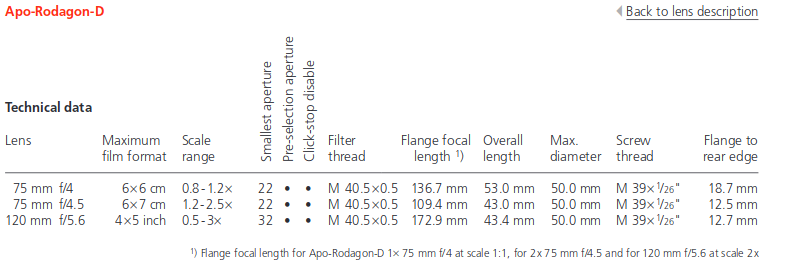
\includegraphics[width=\textwidth]{apo-rodagon-d-1.png}
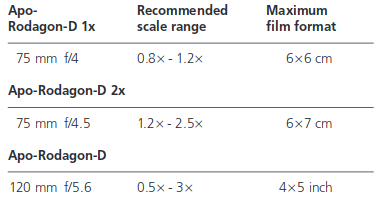
\includegraphics[width=\textwidth]{apo-rodagon-d-2.png}
\end{figure}


\end{document}
